\mode<article>
{
}

\mode<presentation>
{
\usetheme{SystemCoDesigner}
\usenavigationsymbolstemplate{} % uncomment to get rid of navigation symbols

}


%\let\Tiny=\tiny
\usepackage[utf8]{inputenc}
\usepackage{pslatex}
\usepackage{graphicx}
\definecolor{lightgray}{gray}{.9}

\usepackage{booktabs}

\usepackage{makeidx}
\makeindex
\mode<presentation>
{
%\newenvironment{theindex}
%               {\if@twocolumn
%                  \@restonecolfalse
%                \else
%                  \@restonecoltrue
%                \fi
%                \twocolumn[\section*{\indexname}]%
%                \@mkboth{\MakeUppercase\indexname}%
%                        {\MakeUppercase\indexname}%
%                \thispagestyle{plain}\parindent\z@
%                \parskip\z@ \@plus .3\p@\relax
%                \columnseprule \z@
%                \columnsep 35\p@
%                \let\item\@idxitem}
%               {\if@restonecol\onecolumn\else\clearpage\fi}

\newenvironment{theindex}%          environment name
{\let\item\idxitem}% begin code
{}%                    end code
\newcommand\idxitem{\par \hspace*{40pt}}
\newcommand\subitem{\idxitem \hspace*{20pt}}
\newcommand\subsubitem{\idxitem \hspace*{30pt}}
\newcommand\indexspace{\par}
%\renewcommand{\seename}{see}
}

\usepackage{expdlist}
\usepackage{listings}
\lstset{language=C++,showstringspaces=false,breaklines=true,basicstyle=\ttfamily}
\lstset{backgroundcolor=\color{lightgray}}

\mode<presentation>
{
\lstset{commentstyle=\scriptsize\selectfont}
\lstset{basicstyle=\scriptsize\ttfamily\selectfont}
}
%\lstset{commentstyle=\color{blue}}
%\lstset{stringstyle=\color{green}}
%\lstset{keywordstyle=\color{red}}
%\lstset{emph={bool,int,unsigned,char,true,false,void}}
%\lstset{emphstyle=\color{orange}}
\lstset{emph={[2]\#include,\#define,\#ifdef,\#endif}}
\lstset{emphstyle={[2]\color{blue}}}

% macros
\newcommand{\SysteMoC}{\emph{SysteMoC}}
\newcommand{\SystemCoDesigner}{\emph{SystemCoDesigner}}
\newcommand{\VPCs}{\emph{Virtual Processing Components}}
\newcommand{\VPC}{\emph{Virtual Processing Component}}
\newcommand{\concat}{{}^{\smallfrown}}
\newcommand{\length}{\#}



\title{SystemCoDesigner: Performance Modeling Tutorial}
\author{}

%\institute[Hardware/Software Co-Design]{Hardware/Software Co-Design\\University of Erlangen-Nuremberg}
\institute[Hardware/Software Co-Design]{Documentation and examples are available online:\\ http://www.mycodesign.com/research/scd}
\mode<presentation>
{
\university{Friedrich-Alexander University of Erlangen-Nuremberg}
}
\date{Version 1.0}

\AtBeginSubsection[]
{
   \begin{frame}
       \frametitle{Outline}
       \tableofcontents[currentsection,currentsubsections,hideothersubsections]
   \end{frame}
}

\begin{document}

\begin{frame}
  \titlepage
\end{frame}

\begin{frame}
  \frametitle{Outline}
  \tableofcontents[hideallsubsections]
\end{frame}



\section{Introduction}
%%%%%%%%%%%%%%%%%%%%%%%%%%%%%%%%%%%%%%%%%%%%%%%%%%%%%%%%%%%%%%%%%%%%%%%%%%%%%%
%%%%%%%%%%%%%%%%%%%%%%%%%%%%%%%%%%%%%%%%%%%%%%%%%%%%%%%%%%%%%%%%%%%%%%%%%%%%%%
\begin{frame}[t]
\mode<presentation>{\frametitle{\insertsubsection\ }}
\begin{itemize}
\item \SystemCoDesigner{} uses \SysteMoC{} and \VPC\ for functional and performance simulation
\end{itemize}
\begin{itemize}
\item \SysteMoC{} allows for functional modeling and simulation
\end{itemize}

\begin{itemize}
\item \VPC\ (VPC) allow for performance modeling and simulation
\end{itemize}

\begin{itemize}
\item Together, \SysteMoC{} and \VPC\, allow for combined functional and performance simulation
\end{itemize}

\begin{itemize}
\item Both, \SysteMoC{} and \VPC\, are implemented as individual libraries on top of SystemC
\end{itemize}

\end{frame}


%%%%%%%%%%%%%%%%%%%%%%%%%%%%%%%%%%%%%%%%%%%%%%%%%%%%%%%%%%%%%%%%%%%%%%%%%%%%%%
%%%%%%%%%%%%%%%%%%%%%%%%%%%%%%%%%%%%%%%%%%%%%%%%%%%%%%%%%%%%%%%%%%%%%%%%%%%%%%
\begin{frame}[t]
\mode<presentation>{\frametitle{\insertsection\ -- VPC }}
\begin{itemize}
\item A \VPC\ ...
\item ... is a SystemC module
\item ... models task execution times
\item ... models resource contention, scheduling, and arbitration
\end{itemize}

\begin{itemize}
\item A \VPC\ ...
\item ... is not an Instruction Set Simulator
\item ... is not Software
\item ... is not Hardware
\end{itemize}

\begin{itemize}
\item But, a \VPC\ ...
\item ... allows to model a Processor or a HW component
\item ... allows to model a communication resource
\end{itemize}

\end{frame}



%%%%%%%%%%%%%%%%%%%%%%%%%%%%%%%%%%%%%%%%%%%%%%%%%%%%%%%%%%%%%%%%%%%%%%%%%%%%%%
%%%%%%%%%%%%%%%%%%%%%%%%%%%%%%%%%%%%%%%%%%%%%%%%%%%%%%%%%%%%%%%%%%%%%%%%%%%%%%
\begin{frame}[t]
\mode<presentation>{\frametitle{\insertsection\ -- \SysteMoC\ }}

\begin{figure}
\centering
\resizebox{0.7\columnwidth}{!}{\input{vpc-systemoc-fig.tex}}
\end{figure}

\begin{itemize}
\item A functional model in \SysteMoC\ is given by ...
\item ... a set of actors (e.g., Source and Sink)
\item ... a set of communication queues connecting actors 
\end{itemize}
\end{frame}



%%%%%%%%%%%%%%%%%%%%%%%%%%%%%%%%%%%%%%%%%%%%%%%%%%%%%%%%%%%%%%%%%%%%%%%%%%%%%%
%%%%%%%%%%%%%%%%%%%%%%%%%%%%%%%%%%%%%%%%%%%%%%%%%%%%%%%%%%%%%%%%%%%%%%%%%%%%%%
\begin{frame}[t]
\mode<presentation>{\frametitle{\VPC\ }}

\begin{figure}
\centering
\resizebox{0.7\columnwidth}{!}{\input{vpc-systemoc-fig.tex}}
\end{figure}

\begin{itemize}
\item An architecture model in VPC is given by ...
\item ... a set of components (e.g., CPU, Bus, and Mem )
\item ... a mapping of actors and queues to the set of components
\end{itemize}
\end{frame}











\section{Installation Remarks}
%%%%%%%%%%%%%%%%%%%%%%%%%%%%%%%%%%%%%%%%%%%%%%%%%%%%%%%%%%%%%%%%%%%%%%%%%%%%%%
%%
%%%%%%%%%%%%%%%%%%%%%%%%%%%%%%%%%%%%%%%%%%%%%%%%%%%%%%%%%%%%%%%%%%%%%%%%%%%%%%
\subsection{Linux: From Source Code}

%%%%%%%%%%%%%%%%%%%%%%%%%%%%%%%%%%%%%%%%%%%%%%%%%%%%%%%%%%%%%%%%%%%%%%%%%%%%%%
%%%%%%%%%%%%%%%%%%%%%%%%%%%%%%%%%%%%%%%%%%%%%%%%%%%%%%%%%%%%%%%%%%%%%%%%%%%%%%
\begin{frame}[t]
\mode<presentation>{\frametitle{\insertsection\ -- Requirements}}
VPC requirements:
\begin{itemize}
\item A SysteMoC library compiled with VPC support
\item The application needs to be linked with the VPC library
\end{itemize}
library dependencies:
\begin{itemize}
\item CoSupport library (included in the SysteMoC source distribution)
\item Xerces-C++ XML Parser, http://xerces.apache.org/xerces-c/ (Version $\ge$ 2.8.0)
\item Boost C++ library, http://www.boost.org/ (Version $\ge$ 1.35)
\item SystemC library, http://www.systemc.org/ (Version $\ge$ 2.2.0)
\end{itemize}
note:
\begin{itemize}
\item Boost, SystemC, and CoSupport are required for SysteMoC
\item Xerces-C++ is required by the VPC library
\end{itemize}

\end{frame}

%%%%%%%%%%%%%%%%%%%%%%%%%%%%%%%%%%%%%%%%%%%%%%%%%%%%%%%%%%%%%%%%%%%%%%%%%%%%%%
%%%%%%%%%%%%%%%%%%%%%%%%%%%%%%%%%%%%%%%%%%%%%%%%%%%%%%%%%%%%%%%%%%%%%%%%%%%%%%
 % fragile is mandatory for verbatim environments (lstlisting)
 % HACK: use singleslide for correct page numbering
 %  (page_counter+=2 else wise)
 %  this issue seems to be relevant for *pdflatex* only
 % NOTE: the intended usage for *singleslide* is to tell beamer that we use
 %   no overlays (animation)
\begin{frame}[fragile=singleslide]
\mode<presentation>{\frametitle{\insertsubsection}}
\begin{lstlisting}
> cd systemoc-top/
> ls
Support SystemC-VPC SysteMoC Testcases Examples  configure ...
> mkdir obj
> cd obj
> ../configure -C
> make
> (sudo make install)
\end{lstlisting}
\begin{itemize}
\item The source code distribution includes the subdirectories SysteMoC, Support, SystemC-VPC, and some Testcases and Examples
\item Create an obj directory and change the working directory
\item Run the configure script from the source directory
\item Compile the software (and optionally install it)
\end{itemize}
\end{frame}



\section{Virtual Processing Components}
%%%%%%%%%%%%%%%%%%%%%%%%%%%%%%%%%%%%%%%%%%%%%%%%%%%%%%%%%%%%%%%%%%%%%%%%%%%%%%
%%
%%%%%%%%%%%%%%%%%%%%%%%%%%%%%%%%%%%%%%%%%%%%%%%%%%%%%%%%%%%%%%%%%%%%%%%%%%%%%%
\subsection{Functional Model}

%%%%%%%%%%%%%%%%%%%%%%%%%%%%%%%%%%%%%%%%%%%%%%%%%%%%%%%%%%%%%%%%%%%%%%%%%%%%%%
%%%%%%%%%%%%%%%%%%%%%%%%%%%%%%%%%%%%%%%%%%%%%%%%%%%%%%%%%%%%%%%%%%%%%%%%%%%%%%
\begin{frame}[t]
\mode<presentation>{\frametitle{\insertsubsection\ -- SysteMoC Recap}}
\begin{figure}
\centering
\resizebox{0.7\columnwidth}{!}{\input{vpc-systemoc-fig.tex}}
\end{figure}

\begin{itemize}
\item Write a functional model in SysteMoC
\item Two actors, Source and Sink, are connected via a FIFO queue
\item cf. ``SystemCoDesigner: System Programming Tutorial''
\end{itemize}

\end{frame}


%%%%%%%%%%%%%%%%%%%%%%%%%%%%%%%%%%%%%%%%%%%%%%%%%%%%%%%%%%%%%%%%%%%%%%%%%%%%%%
%%%%%%%%%%%%%%%%%%%%%%%%%%%%%%%%%%%%%%%%%%%%%%%%%%%%%%%%%%%%%%%%%%%%%%%%%%%%%%
 % fragile is mandatory for verbatim environments (lstlisting)
 % HACK: use singleslide for correct page numbering
%  (page_counter+=2 else wise)
 %  this issue seems to be relevant for *pdflatex* only
 % NOTE: the intended usage for *singleslide* is to tell beamer that we use
 %   no overlays (animation)
\begin{frame}[fragile=singleslide]
\mode<presentation>{\frametitle{\insertsubsection}}
\begin{lstlisting}
//file vpc_source_sink.cpp
#include <iostream>
#include <systemoc/smoc_moc.hpp>
static const std::string MESSAGE = "Hello SysteMoC!";

class Source : public smoc_actor{
public:
  smoc_port_out<char> out;

  Source(sc_module_name name) : smoc_actor(name, start),
    count(0), size(MESSAGE.size()), message(MESSAGE) {
    start = GUARD(Source::hasToken) >>
      out(1)                        >>
      CALL(Source::src)             >> start;
  }
\end{lstlisting}
\begin{itemize}
\item The Source actor has an output port with data type \lstinline!char!
\item A single FSM transition is used to produce one data token per actor firing
\end{itemize}
\end{frame}


%%%%%%%%%%%%%%%%%%%%%%%%%%%%%%%%%%%%%%%%%%%%%%%%%%%%%%%%%%%%%%%%%%%%%%%%%%%%%%
%%%%%%%%%%%%%%%%%%%%%%%%%%%%%%%%%%%%%%%%%%%%%%%%%%%%%%%%%%%%%%%%%%%%%%%%%%%%%%
\begin{frame}[fragile=singleslide]
\mode<presentation>{\frametitle{\insertsubsection}}
\begin{lstlisting}
//file vpc_source_sink.cpp cont'd
private:
  smoc_firing_state start;   // states
  unsigned int count, size;  // variables (functional state)
  const std::string message; //

  bool hasToken() const {
    return count < size;
  } // guard

  void src() {
    std::cerr << this->name() << "> @ " << sc_time_stamp()
        << "\tsend: \'" << message[count] << "\'" << std::endl;

    out[0] = message[count++];
  } // action
};
\end{lstlisting}
\begin{itemize}
\item A function \lstinline!src()! is used to produce data tokens
\item A guard \lstinline!hasToken()! is used to check if the transition can be fired
\end{itemize}
\end{frame}


%%%%%%%%%%%%%%%%%%%%%%%%%%%%%%%%%%%%%%%%%%%%%%%%%%%%%%%%%%%%%%%%%%%%%%%%%%%%%%
%%%%%%%%%%%%%%%%%%%%%%%%%%%%%%%%%%%%%%%%%%%%%%%%%%%%%%%%%%%%%%%%%%%%%%%%%%%%%%
\begin{frame}[fragile=singleslide]
\mode<presentation>{\frametitle{\insertsubsection}}
\begin{lstlisting}
//file vpc_source_sink.cpp cont'd
class Sink : public smoc_actor {
public:
  smoc_port_in<char> in;

  Sink(sc_module_name name) // actor constructor
  : smoc_actor(name, start) {
    start = in(1) >> CALL(Sink::sink) >> start;
  }
private:
  smoc_firing_state start;

  void sink() {
    std::cout << this->name() << "> @ " << sc_time_stamp()
        << "\trecv: \'" << in[0] << "\'" << std::endl;
  }
};
\end{lstlisting}
\begin{itemize}
\item The Sink actor receives and consumes the data token
\item \lstinline!this->name()! returns the entire hierarchical name of the actor
\end{itemize}
\end{frame}


%%%%%%%%%%%%%%%%%%%%%%%%%%%%%%%%%%%%%%%%%%%%%%%%%%%%%%%%%%%%%%%%%%%%%%%%%%%%%%
%%%%%%%%%%%%%%%%%%%%%%%%%%%%%%%%%%%%%%%%%%%%%%%%%%%%%%%%%%%%%%%%%%%%%%%%%%%%%%
\begin{frame}[fragile=singleslide]
\mode<presentation>{\frametitle{\insertsubsection}}
\begin{lstlisting}
//file vpc_source_sink.cpp cont'd
class NetworkGraph : public smoc_graph {
public:
  NetworkGraph(sc_module_name name)
   : smoc_graph(name), source("Source"), sink("Sink") {
    smoc_fifo<char> fifo("queue", 4);
    fifo.connect(source.out).connect(sink.in); // connect actors
  }
private:
  Source source; // actors
  Sink sink;
};
int sc_main(int argc, char **argv){
  NetworkGraph top("top"); // create network graph
  smoc_scheduler_top sched(top);
  sc_start(); // start simulation (SystemC)
  return 0;
}
\end{lstlisting}
\begin{itemize}
\item Source and Sink are connected via a queue (queue size = 4)
\item VPC usage is easier with (unique) symbolic queue names
\end{itemize}
\end{frame}


%%%%%%%%%%%%%%%%%%%%%%%%%%%%%%%%%%%%%%%%%%%%%%%%%%%%%%%%%%%%%%%%%%%%%%%%%%%%%%
%%%%%%%%%%%%%%%%%%%%%%%%%%%%%%%%%%%%%%%%%%%%%%%%%%%%%%%%%%%%%%%%%%%%%%%%%%%%%%
\begin{frame}[fragile=singleslide]
\mode<presentation>{\frametitle{\insertsubsection}}
\begin{lstlisting}
> ./vpc-src-sink

             SystemC 2.2.0 --- Dec 15 2008 13:19:05
        Copyright (c) 1996-2006 by all Contributors
                    ALL RIGHTS RESERVED            
top.Source> @ 0 s       send: 'H'
top.Sink> @ 0 s recv: 'H'
top.Source> @ 0 s       send: 'e'
top.Sink> @ 0 s recv: 'e'
top.Source> @ 0 s       send: 'l'
top.Sink> @ 0 s recv: 'l'
top.Source> @ 0 s       send: 'l'
top.Sink> @ 0 s recv: 'l'
top.Source> @ 0 s       send: 'o'
top.Sink> @ 0 s recv: 'o'
...
[VPC] overall simulated time: 0 s
\end{lstlisting}
\begin{itemize}
\item Compile source code and run functional simulation
\item No timing is simulated in the functional model
\end{itemize}
\end{frame}


%%%%%%%%%%%%%%%%%%%%%%%%%%%%%%%%%%%%%%%%%%%%%%%%%%%%%%%%%%%%%%%%%%%%%%%%%%%%%%
%%%%%%%%%%%%%%%%%%%%%%%%%%%%%%%%%%%%%%%%%%%%%%%%%%%%%%%%%%%%%%%%%%%%%%%%%%%%%%
\begin{frame}[fragile=singleslide]
\mode<presentation>{\frametitle{\insertsubsection}}
\begin{itemize}
\item When compiled with VPC, the SysteMoC functional simulation forwards actor execution and communication events to the VPC library
\item A performance simulation for those events will take place if an architecture model is given to the VPC simulation
\item The architecture model is given by an XML configuration file
\item A pure functional simulation without timing is performed if no architecture model is given
\end{itemize}
\end{frame}


%%%%%%%%%%%%%%%%%%%%%%%%%%%%%%%%%%%%%%%%%%%%%%%%%%%%%%%%%%%%%%%%%%%%%%%%%%%%%%
%%
%%%%%%%%%%%%%%%%%%%%%%%%%%%%%%%%%%%%%%%%%%%%%%%%%%%%%%%%%%%%%%%%%%%%%%%%%%%%%%
\subsection{Architecture Model}


\lstset{language=XML}
%%%%%%%%%%%%%%%%%%%%%%%%%%%%%%%%%%%%%%%%%%%%%%%%%%%%%%%%%%%%%%%%%%%%%%%%%%%%%%
%%%%%%%%%%%%%%%%%%%%%%%%%%%%%%%%%%%%%%%%%%%%%%%%%%%%%%%%%%%%%%%%%%%%%%%%%%%%%%
\begin{frame}[fragile=singleslide]
\mode<presentation>{\frametitle{\insertsubsection}}
\begin{lstlisting}
<?xml version="1.0"?>
<!DOCTYPE vpcconfiguration SYSTEM "vpc.dtd">
<vpcconfiguration>
 <resources>
  ...
 </resources>

 <mappings>
  ...
 </mappings>

 <topology>
  ...
 </topology>
</vpcconfiguration>
\end{lstlisting}
\begin{itemize}
\item Write a VPC configuration (XML file \lstinline!src-snk.vpc.xml!)
\item \lstinline!.vpc.xml! is the preferred file name suffix
\item The document type definition is given in the file (\lstinline!vpc.dtd!)
\end{itemize}
\end{frame}


%%%%%%%%%%%%%%%%%%%%%%%%%%%%%%%%%%%%%%%%%%%%%%%%%%%%%%%%%%%%%%%%%%%%%%%%%%%%%%
%%%%%%%%%%%%%%%%%%%%%%%%%%%%%%%%%%%%%%%%%%%%%%%%%%%%%%%%%%%%%%%%%%%%%%%%%%%%%%
\begin{frame}[fragile=singleslide]
\mode<presentation>{\frametitle{\insertsubsection}}
\index{vpcconfiguration@\lstinline{<vpcconfiguration>}}
\index{resources@\lstinline{<resources>}}
\begin{lstlisting}
<?xml version="1.0"?>
<!DOCTYPE vpcconfiguration SYSTEM "vpc.dtd">
<vpcconfiguration>
 <resources>
  ...
 </resources>

 <mappings>
  ...
 </mappings>

 <topology>
  ...
 </topology>
</vpcconfiguration>
\end{lstlisting}
\begin{itemize}
\item \lstinline!<vpcconfiguration>! is the XML root element of a VPC configuration
\item It contains the elements \lstinline!<resources>!, \lstinline!<mappings>!, and \lstinline!<topology>!
\end{itemize}
\end{frame}


%%%%%%%%%%%%%%%%%%%%%%%%%%%%%%%%%%%%%%%%%%%%%%%%%%%%%%%%%%%%%%%%%%%%%%%%%%%%%%
%%%%%%%%%%%%%%%%%%%%%%%%%%%%%%%%%%%%%%%%%%%%%%%%%%%%%%%%%%%%%%%%%%%%%%%%%%%%%%
\begin{frame}[fragile=singleslide]
\mode<presentation>{\frametitle{\insertsubsection}}
\begin{lstlisting}
 <resources>
  <component name="CPU" scheduler="FCFS">
   <attribute type="transfer_delay" value="20 ns" />
  </component>
  <component name="Bus" scheduler="FCFS">
   <attribute type="transfer_delay" value="80 ns" />
  </component>
  <component name="Mem" scheduler="FCFS">
   <attribute type="transfer_delay" value="20 ns" />
  </component>
 </resources>
\end{lstlisting}
\index{resources@\lstinline{<resources>}}
\index{component@\lstinline{<component>}}
\index{scheduler@\lstinline{scheduler}}
\begin{itemize}
\item The \lstinline!<resources>! element contains nested \lstinline!<component>! elements
\item An element \lstinline!<component>! defines a (Virtual Processing) Component
\item Each Component has a name and a scheduler given by the XML attributes \lstinline!name! and \lstinline!scheduler!
\end{itemize}
\end{frame}


%%%%%%%%%%%%%%%%%%%%%%%%%%%%%%%%%%%%%%%%%%%%%%%%%%%%%%%%%%%%%%%%%%%%%%%%%%%%%%
%%%%%%%%%%%%%%%%%%%%%%%%%%%%%%%%%%%%%%%%%%%%%%%%%%%%%%%%%%%%%%%%%%%%%%%%%%%%%%
\begin{frame}[fragile=singleslide]
\mode<presentation>{\frametitle{\insertsubsection\ -- Attributes}}
\begin{lstlisting}
 <resources>
  <component name="CPU" scheduler="FCFS">
   <attribute type="transfer_delay" value="20 ns" />
  </component>
  <component name="Bus" scheduler="FCFS">
   <attribute type="transfer_delay" value="80 ns" />
  </component>
  <component name="Mem" scheduler="FCFS">
   <attribute type="transfer_delay" value="20 ns" />
  </component>
 </resources>
\end{lstlisting}
\index{component@\lstinline{<component>}}
\begin{itemize}
\item Components may have attributes (nested \lstinline!<attribute>! elements)
\item An attributes is defined by a type and a value (\lstinline!<attribute type="..." value="..." />!)
\item E.g., an attribute \lstinline!transfer_delay! refers to the communication time required for one token, if the communication route includes this component (cf. \lstinline!route!)
\end{itemize}
\end{frame}


%%%%%%%%%%%%%%%%%%%%%%%%%%%%%%%%%%%%%%%%%%%%%%%%%%%%%%%%%%%%%%%%%%%%%%%%%%%%%%
%%%%%%%%%%%%%%%%%%%%%%%%%%%%%%%%%%%%%%%%%%%%%%%%%%%%%%%%%%%%%%%%%%%%%%%%%%%%%%
\begin{frame}[fragile=singleslide]
\mode<presentation>{\frametitle{\insertsubsection\ -- Mappings}}
\begin{lstlisting}
 <mappings>
  <mapping source="top.Source" target="CPU">
   <timing dii="10 us" latency="10 us" />
   <timing fname="Source::src" dii="10 us" latency="10 us" />
  </mapping>
  <mapping source="top.Sink" target="CPU">
   <timing delay="10 us" />
   <timing fname="Sink::sink" delay="10 us" />
  </mapping>
 </mappings>
\end{lstlisting}
\index{mappings@\lstinline{<mappings>}}
\index{mapping@\lstinline{<mapping>}}
\begin{itemize}
\item \lstinline!mapping! elements are nested inside the \lstinline!mappings! element
\item Used to define the mapping of actors to components
\item The attribute \lstinline!source! defines the hierarchical actor name
\item The attribute \lstinline!target! defines the Component name (cf. \lstinline!<component>!)
\end{itemize}
\end{frame}


%%%%%%%%%%%%%%%%%%%%%%%%%%%%%%%%%%%%%%%%%%%%%%%%%%%%%%%%%%%%%%%%%%%%%%%%%%%%%%
%%%%%%%%%%%%%%%%%%%%%%%%%%%%%%%%%%%%%%%%%%%%%%%%%%%%%%%%%%%%%%%%%%%%%%%%%%%%%%
\begin{frame}[fragile=singleslide]
\mode<presentation>{\frametitle{\insertsubsection\ -- Timing}}
\begin{lstlisting}
 <mappings>
  <mapping source="top.Source" target="CPU">
   <timing dii="10 us" latency="10 us" />
   <timing fname="Source::src" dii="10 us" latency="10 us" />
  </mapping>
  <mapping source="top.Sink" target="CPU">
   <timing delay="10 us" />
   <timing fname="Sink::sink" delay="10 us" />
  </mapping>
 </mappings>
\end{lstlisting}
\index{timing@\lstinline{<timing>}}
\begin{itemize}
\item A \lstinline!timing! element defines the execution times for a mapping
\item The execution time is given either
\begin{itemize}
\item By a \lstinline!dii! and  \lstinline!latency! attribute
\item Or by a \lstinline!delay! attribute
\end{itemize}
\item Thereby \lstinline!delay="X"! is a short cut for \lstinline!dii="X" latency="X"!
\item \lstinline!dii! and \lstinline!latency! are constraint to: $(0 < dii \le lat) \vee (0=dii=lat)$
\end{itemize}
\vfill
\end{frame}


%%%%%%%%%%%%%%%%%%%%%%%%%%%%%%%%%%%%%%%%%%%%%%%%%%%%%%%%%%%%%%%%%%%%%%%%%%%%%%
%%%%%%%%%%%%%%%%%%%%%%%%%%%%%%%%%%%%%%%%%%%%%%%%%%%%%%%%%%%%%%%%%%%%%%%%%%%%%%
\begin{frame}[fragile=singleslide]
\mode<presentation>{\frametitle{\insertsubsection\ -- Timing}}
\begin{lstlisting}
 <mappings>
  <mapping source="top.Source" target="CPU">
   <timing dii="10 us" latency="10 us" />
   <timing fname="Source::src" dii="10 us" latency="10 us" />
  </mapping>
  <mapping source="top.Sink" target="CPU">
   <timing delay="10 us" />
   <timing fname="Sink::sink" delay="10 us" />
  </mapping>
 </mappings>
\end{lstlisting}
\index{timing@\lstinline{<timing>}}
\index{fname@\lstinline{fname}}
\begin{itemize}
\item The attribute \lstinline!fname! is optional,
\item The default timing of an actor is given without \lstinline!fname!
\end{itemize}
\vfill
\end{frame}


%%%%%%%%%%%%%%%%%%%%%%%%%%%%%%%%%%%%%%%%%%%%%%%%%%%%%%%%%%%%%%%%%%%%%%%%%%%%%%
%%%%%%%%%%%%%%%%%%%%%%%%%%%%%%%%%%%%%%%%%%%%%%%%%%%%%%%%%%%%%%%%%%%%%%%%%%%%%%
\begin{frame}[fragile=singleslide]
\mode<presentation>{\frametitle{\insertsubsection\ -- Timing}}
\begin{lstlisting}
 <mappings>
  <mapping source="top.Source" target="CPU">
   <timing dii="10 us" latency="10 us" />
   <timing fname="Source::src" dii="10 us" latency="10 us" />
  </mapping>
  <mapping source="top.Sink" target="CPU">
   <timing delay="10 us" />
   <timing fname="Sink::sink" delay="10 us" />
  </mapping>
 </mappings>
\end{lstlisting}
\index{timing@\lstinline{<timing>}}
\index{fname@\lstinline{fname}}
\begin{itemize}
\item With \lstinline!fname! individual timings are specified for the given function names (names given by SysteMoC's \lstinline!CALL(...)! and \lstinline!GUARD(...)! macros, cf. ``SystemCoDesigner: System Programming Tutorial'')
\item The execution time (dii and latency) of a transition is the sum of function times for all guards and actions referred by this transition.
\item Timing is simulated only if the transition is executed, i.e., the guards evaluate to true.
\end{itemize}
\vfill
\end{frame}


%%%%%%%%%%%%%%%%%%%%%%%%%%%%%%%%%%%%%%%%%%%%%%%%%%%%%%%%%%%%%%%%%%%%%%%%%%%%%%
%%%%%%%%%%%%%%%%%%%%%%%%%%%%%%%%%%%%%%%%%%%%%%%%%%%%%%%%%%%%%%%%%%%%%%%%%%%%%%
\begin{frame}[fragile=singleslide]
\mode<presentation>{\frametitle{\insertsubsection\ -- Topology}}
\begin{lstlisting}
 <topology>
  <route  source="top.Source" destination="queue">
   <hop name="CPU">  </hop>
   <hop name="Bus">  </hop>
   <hop name="Mem">  </hop>
  </route>
  <route  source="queue" destination="top.Sink">
   <hop name="Mem">  </hop>
   <hop name="Bus">  </hop>
   <hop name="CPU">  </hop>
  </route>
 </topology>
\end{lstlisting}
\index{topology@\lstinline{<topology>}}
\index{route@\lstinline{<route>}}
\begin{itemize}
\item The  \lstinline!<topology>! section defines the multi-hop communication routes
\item The \lstinline!<topology>! is defined by nested \lstinline!<route>! elements
\item For each connection between an actor and a channel a  \lstinline!<route>! may be defined
\end{itemize}
\end{frame}


%%%%%%%%%%%%%%%%%%%%%%%%%%%%%%%%%%%%%%%%%%%%%%%%%%%%%%%%%%%%%%%%%%%%%%%%%%%%%%
%%%%%%%%%%%%%%%%%%%%%%%%%%%%%%%%%%%%%%%%%%%%%%%%%%%%%%%%%%%%%%%%%%%%%%%%%%%%%%
\begin{frame}[fragile=singleslide]
\mode<presentation>{\frametitle{\insertsubsection\ -- Route}}
\begin{lstlisting}
 <topology>
  <route  source="top.Source" destination="queue">
   <hop name="CPU">  </hop>
   <hop name="Bus">  </hop>
   <hop name="Mem">  </hop>
  </route>
  <route  source="queue" destination="top.Sink">
   <hop name="Mem">  </hop>
   <hop name="Bus">  </hop>
   <hop name="CPU">  </hop>
  </route>
 </topology>
\end{lstlisting}
\index{route@\lstinline{<route>}}
\index{hop@\lstinline{<hop>}}
\begin{itemize}
\item A \lstinline!<route>! is defined by nested \lstinline!<hop>! elements
\item A route has a \lstinline!source! and a \lstinline!target! attribute
\item Source and target form a pair (actor, channel) or (channel, actor)
\item Suggestion: use symbolic queue names in the SysteMoC model
\item Else: queue names are concatenations of connected actor names
\end{itemize}
\end{frame}

%%%%%%%%%%%%%%%%%%%%%%%%%%%%%%%%%%%%%%%%%%%%%%%%%%%%%%%%%%%%%%%%%%%%%%%%%%%%%%
%%%%%%%%%%%%%%%%%%%%%%%%%%%%%%%%%%%%%%%%%%%%%%%%%%%%%%%%%%%%%%%%%%%%%%%%%%%%%%
\begin{frame}[t]
\mode<presentation>{\frametitle{\insertsubsection\ -- Hops}}
\begin{figure}
\centering
\resizebox{0.7\columnwidth}{!}{\input{vpc-systemoc-fig.tex}}
\end{figure}
\index{hop@\lstinline{<hop>}}

\begin{itemize}
\item The \lstinline!<hop>! elements of a route refer to Components (by name)
\item E.g., the route for actor Source writing the queue involves the hops CPU, Bus, and Mem
\end{itemize}

\end{frame}




%%%%%%%%%%%%%%%%%%%%%%%%%%%%%%%%%%%%%%%%%%%%%%%%%%%%%%%%%%%%%%%%%%%%%%%%%%%%%%
%%
%%%%%%%%%%%%%%%%%%%%%%%%%%%%%%%%%%%%%%%%%%%%%%%%%%%%%%%%%%%%%%%%%%%%%%%%%%%%%%
\subsection{Performance Simulation}


%%%%%%%%%%%%%%%%%%%%%%%%%%%%%%%%%%%%%%%%%%%%%%%%%%%%%%%%%%%%%%%%%%%%%%%%%%%%%%
%%%%%%%%%%%%%%%%%%%%%%%%%%%%%%%%%%%%%%%%%%%%%%%%%%%%%%%%%%%%%%%%%%%%%%%%%%%%%%
\begin{frame}[fragile=singleslide]
\mode<presentation>{\frametitle{\insertsubsection}}
\begin{lstlisting}
> setenv VPCCONFIGURATION src-snk.vpc.xml
> ./vpc-src-sink

             SystemC 2.2.0 --- Dec 15 2008 13:19:05
        Copyright (c) 1996-2006 by all Contributors
                    ALL RIGHTS RESERVED            
top.Source> @ 0 s       send: 'H'
top.Source> @ 10 us     send: 'e'
top.Sink> @ 10120 ns    recv: 'H'
top.Source> @ 20020 ns  send: 'l'
top.Source> @ 30060 ns  send: 'l'
top.Sink> @ 40060 ns    recv: 'e'
top.Source> @ 50080 ns  send: 'o'
top.Sink> @ 70120 ns    recv: 'l'
...
[VPC] overall simulated time: 300900 ns
\end{lstlisting}
\begin{itemize}
\item Set environment variable \lstinline!VPCCONFIGURATION! to the configuration file and run simulation
\item Timing is simulated and VPC reports overall simulation time 
\end{itemize}
\end{frame}


%%%%%%%%%%%%%%%%%%%%%%%%%%%%%%%%%%%%%%%%%%%%%%%%%%%%%%%%%%%%%%%%%%%%%%%%%%%%%%
%%%%%%%%%%%%%%%%%%%%%%%%%%%%%%%%%%%%%%%%%%%%%%%%%%%%%%%%%%%%%%%%%%%%%%%%%%%%%%
\begin{frame}[fragile=singleslide]
\mode<presentation>{\frametitle{\insertsubsection\ -- Simulation Trace}}
\begin{lstlisting}
$timescale
     1 ns
$end
$scope module sc $end
$var wire    8  aaa  msg_top.Source_2_queue [7:0]  $end
$var wire    8  aab  msg_queue_2_top.Sink [7:0]  $end
$upscope $end
$enddefinitions  $end
$dumpvars
b100000 aaa
b100000 aab
$end

#10020
b1010010 aaa
\end{lstlisting}
\begin{itemize}
\item The simulation is traced in Value Change Dump files
\item A VCD file is created for each component (cf. \lstinline!<resource>!)
\item VCD files can be visualized, e.g., using GTKWave or Modelsim
\end{itemize}
\end{frame}


%%%%%%%%%%%%%%%%%%%%%%%%%%%%%%%%%%%%%%%%%%%%%%%%%%%%%%%%%%%%%%%%%%%%%%%%%%%%%%
%%%%%%%%%%%%%%%%%%%%%%%%%%%%%%%%%%%%%%%%%%%%%%%%%%%%%%%%%%%%%%%%%%%%%%%%%%%%%%
\begin{frame}[t]
\mode<presentation>{\frametitle{\insertsubsection\ -- Simulation Trace}}
\begin{figure}
\centering
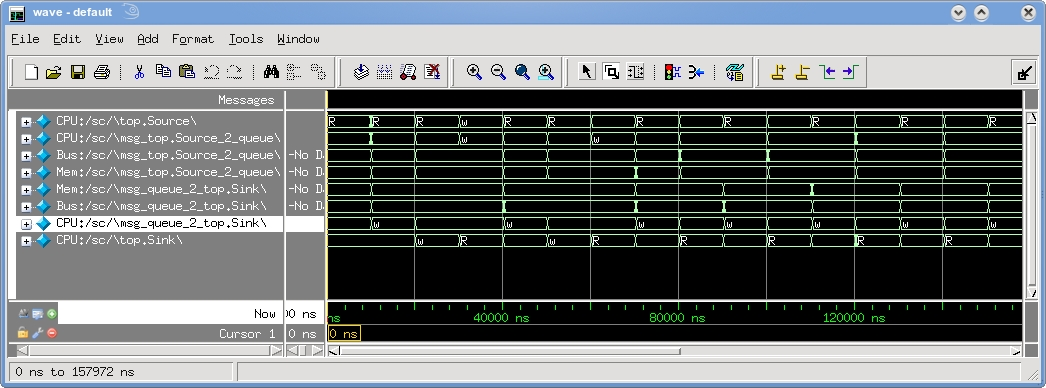
\includegraphics[width=\columnwidth]{vcd-trace0.jpg}
\end{figure}

\begin{itemize}
\item Signal values represent ASCII coded characters (radix = ASCII)
\item Each signal represents a task (an actor or a communication message)
\end{itemize}

\end{frame}


%%%%%%%%%%%%%%%%%%%%%%%%%%%%%%%%%%%%%%%%%%%%%%%%%%%%%%%%%%%%%%%%%%%%%%%%%%%%%%
%%%%%%%%%%%%%%%%%%%%%%%%%%%%%%%%%%%%%%%%%%%%%%%%%%%%%%%%%%%%%%%%%%%%%%%%%%%%%%
\begin{frame}[t]
\mode<presentation>{\frametitle{\insertsubsection\ -- Simulation Trace}}
\begin{figure}
\centering
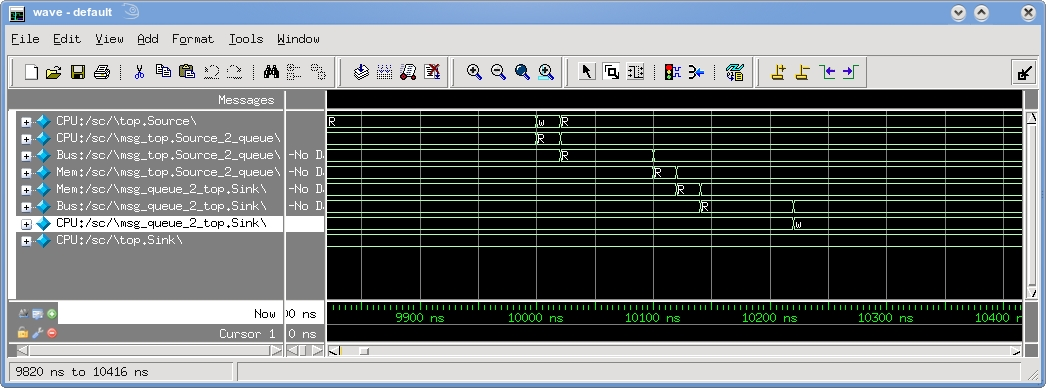
\includegraphics[width=\columnwidth]{vcd-trace1.jpg}
\end{figure}

\begin{itemize}
\item "R" or "r" means a task is executed (running)
\item "W" or "w" means a task is ready for execution but preempted (waiting)
\item "B" or "b" means a task is blocked during communication
\end{itemize}

\end{frame}


%%%%%%%%%%%%%%%%%%%%%%%%%%%%%%%%%%%%%%%%%%%%%%%%%%%%%%%%%%%%%%%%%%%%%%%%%%%%%%
%%
%%%%%%%%%%%%%%%%%%%%%%%%%%%%%%%%%%%%%%%%%%%%%%%%%%%%%%%%%%%%%%%%%%%%%%%%%%%%%%
\subsection{Reference Manual}


%%%%%%%%%%%%%%%%%%%%%%%%%%%%%%%%%%%%%%%%%%%%%%%%%%%%%%%%%%%%%%%%%%%%%%%%%%%%%%
%%%%%%%%%%%%%%%%%%%%%%%%%%%%%%%%%%%%%%%%%%%%%%%%%%%%%%%%%%%%%%%%%%%%%%%%%%%%%%
\begin{frame}[fragile=singleslide]
\mode<presentation>{\frametitle{\insertsubsection\ -- Scheduler}}
\index{scheduler@\lstinline{scheduler}}
\begin{lstlisting}
  <component name="CPU" scheduler="PS">
  ...
  <mapping source="top.Sink" target="CPU">
   <attribute type="priority" value="1" />
\end{lstlisting}
\begin{itemize}
\item VPC includes several different schedulers
\item Most scheduler require additional attributes assigned to mappings and/or to components
\item E.g., a priority scheduler requires priority values assigned to mappings
\end{itemize}
\begin{lstlisting}
  <component name="CPU" scheduler="RR">
   <attribute type="timeslice" value="10 ns" />
  ...
  <mapping source="top.Sink" target="CPU">
\end{lstlisting}
\begin{itemize}
\item The round robin scheduler requires a timeslice attribute assigned to the component
\end{itemize}
\end{frame}


%%%%%%%%%%%%%%%%%%%%%%%%%%%%%%%%%%%%%%%%%%%%%%%%%%%%%%%%%%%%%%%%%%%%%%%%%%%%%%
%%%%%%%%%%%%%%%%%%%%%%%%%%%%%%%%%%%%%%%%%%%%%%%%%%%%%%%%%%%%%%%%%%%%%%%%%%%%%%
\begin{frame}[fragile=singleslide]
\mode<presentation>{\frametitle{\insertsubsection\ -- Scheduler}}
\index{scheduler@\lstinline{scheduler}}
\begin{tabular}{llcc}
\toprule
&& \multicolumn{2}{c}{Required Attributes} \\
\cmidrule(r){3-4}
Scheduler & XML name & Component & Mapping \\
\midrule
First Come First Served      & \lstinline!FCFS!    & &  \\
Priority Scheduler           & \lstinline!PSNOPRE! & & \lstinline!priority! \\
Preemptive Priority Scheduler& \lstinline!PS!      & & \lstinline!priority! \\
Round Robin                  & \lstinline!RR! & \lstinline!timeslice! & \lstinline!priority!  \\
Time Division Multiple Access& \lstinline!TDMA!    & \emph{*} & \\
FlexRay                      & \lstinline!FlexRay! & \emph{*} & \\
\bottomrule
\end{tabular}

\begin{itemize}
\item[*] TDMA and FleyRay scheduler require complex attribute structures
\end{itemize}
\end{frame}


%%%%%%%%%%%%%%%%%%%%%%%%%%%%%%%%%%%%%%%%%%%%%%%%%%%%%%%%%%%%%%%%%%%%%%%%%%%%%%
%%%%%%%%%%%%%%%%%%%%%%%%%%%%%%%%%%%%%%%%%%%%%%%%%%%%%%%%%%%%%%%%%%%%%%%%%%%%%%
\begin{frame}[fragile=singleslide]
\mode<presentation>{\frametitle{\insertsubsection\ -- Hop}}
\index{hop@\lstinline{<hop>}}
\begin{lstlisting}
  <route  source="top.Source" destination="queue">
   <hop name="CPU">  </hop>
   <hop name="Bus">  <timing dii="1000 us" latency="1000 us" />  </hop>
   <hop name="Mem">  </hop>
  </route>
\end{lstlisting}
\begin{itemize}
\item Per default the timing of a \lstinline!hop! is defined by the components attribute \lstinline!transfer_delay!
\item A nested \lstinline!<timing>! element may be used to override the default
\end{itemize}
\end{frame}





%%%%%%%%%%%%%%%%%%%%%%%%%%%%%%%%%%%%%%%%%%%%%%%%%%%%%%%%%%%%%%%%%%%%%%%%%%%%%%
% Section Remarks
%%%%%%%%%%%%%%%%%%%%%%%%%%%%%%%%%%%%%%%%%%%%%%%%%%%%%%%%%%%%%%%%%%%%%%%%%%%%%%
\section{Remarks}
\begin{frame}
  \frametitle{Outline}
  \tableofcontents[currentsection,hideallsubsections]
\end{frame}


%%%%%%%%%%%%%%%%%%%%%%%%%%%%%%%%%%%%%%%%%%%%%%%%%%%%%%%%%%%%%%%%%%%%%%%%%%%%%%
% Contact
%%%%%%%%%%%%%%%%%%%%%%%%%%%%%%%%%%%%%%%%%%%%%%%%%%%%%%%%%%%%%%%%%%%%%%%%%%%%%%
\begin{frame}
\mode<presentation>{\frametitle{Contact}}
\begin{description}[\breaklabel\setleftmargin{60pt}\setlabelstyle{\color{beamer@SystemCoDesigner@color}}]
\item[Contact Persons:]
Christian Haubelt, Jürgen Teich
\item[Email:] codesigner@mycodesign.com
\item[Address:]
Hardware/Software Co-Design\\
Department of Computer Science\\
University of Erlangen-Nuremberg\\
Am Weichselgarten 3\\
91058 Erlangen, Germany
%\item[History:]
%Version 1.0:  2009/10/01
\end{description}
\end{frame}




%%%%%%%%%%%%%%%%%%%%%%%%%%%%%%%%%%%%%%%%%%%%%%%%%%%%%%%%%%%%%%%%%%%%%%%%%%%%%%
% Credits
%%%%%%%%%%%%%%%%%%%%%%%%%%%%%%%%%%%%%%%%%%%%%%%%%%%%%%%%%%%%%%%%%%%%%%%%%%%%%%
\begin{frame}
\mode<presentation>{\frametitle{Credits}}
\begin{description}[\breaklabel\setleftmargin{60pt}\setlabelstyle{\color{beamer@SystemCoDesigner@color}}]
\item[SysteMoC Development Team:]
Joachim Falk, Jens Gladigau, Martin Streubühr, Christian Zebelein
\item[VPC Development Team:]
Martin Streubühr, Sebastian Graf
\item[SystemCoDesigner Contributors:]
Joachim Falk, Michael Glass, Jens Gladigau, Joachim Keinert, Martin Lukasiewycz, Felix Reimann, Thomas Schlichter, Thilo Streichert, Martin Streubühr, Christian Zebelein, Christian Haubelt, Jürgen Teich
\end{description}
\end{frame}


%%%%%%%%%%%%%%%%%%%%%%%%%%%%%%%%%%%%%%%%%%%%%%%%%%%%%%%%%%%%%%%%%%%%%%%%%%%%%%
% Contact
%%%%%%%%%%%%%%%%%%%%%%%%%%%%%%%%%%%%%%%%%%%%%%%%%%%%%%%%%%%%%%%%%%%%%%%%%%%%%%
\begin{frame}
\mode<presentation>{\frametitle{Document Info}}
\begin{description}[\breaklabel\setleftmargin{60pt}\setlabelstyle{\color{beamer@SystemCoDesigner@color}}]
\item[Authors:]
Martin Streubühr, Sebastian Graf
\item[Document Release:]
August 25, 2010
\item[Version History:]
August 25, 2010: Version 1.0
\end{description}
\end{frame}




%%%%%%%%%%%%%%%%%%%%%%%%%%%%%%%%%%%%%%%%%%%%%%%%%%%%%%%%%%%%%%%%%%%%%%%%%%%%%%
% Section: Index
%%%%%%%%%%%%%%%%%%%%%%%%%%%%%%%%%%%%%%%%%%%%%%%%%%%%%%%%%%%%%%%%%%%%%%%%%%%%%%
\section{Index}
\begin{frame}
\mode<presentation>{\frametitle{Index}}
{\footnotesize
\printindex
}
\end{frame}


\end{document}

